\documentclass[12pt]{article}
\usepackage{amsmath}
\usepackage{times}
\usepackage{graphicx}
\usepackage{color}
\usepackage{multirow}

\usepackage[authoryear]{natbib}

\usepackage{rotating}
\usepackage{bbm}
\usepackage{latexsym}

%%% margins
\textheight 23.4cm
\textwidth 14.65cm
\oddsidemargin 0.375in
\evensidemargin 0.375in
\topmargin  -0.55in

\renewcommand{\baselinestretch}{2}

\interfootnotelinepenalty=10000

% Different font in captions
\newcommand{\captionfonts}{\normalsize}

\makeatletter
\long\def\@makecaption#1#2{%
  \renewcommand{\baselinestretch}{1}% EH: stop captions running off the bottom of the page
  \vskip\abovecaptionskip
  \sbox\@tempboxa{{\captionfonts #1: #2}}%
  \ifdim \wd\@tempboxa >\hsize
    {\captionfonts #1: #2\par}
  \else
    \hbox to\hsize{\hfil\box\@tempboxa\hfil}%
  \fi
  \vskip\belowcaptionskip}
\makeatother
%%%%%

\usepackage{nameref}

\graphicspath{{../figures/}}
%% \newcommand{\hidefigures}{\relax}

\begin{document}
\hspace{13.9cm}

\ \vspace{20mm}\\

{\LARGE The competing benefits of noise and heterogeneity in neural coding}

\ \\
{\bf \large Eric Hunsberger$^{\displaystyle 1}$, Matthew Scott$^{\displaystyle 2}$, Chris Eliasmith$^{\displaystyle 1}$}\\
{$^{\displaystyle 1}$Centre for Theoretical Neuroscience, University of Waterloo, Waterloo, Canada.}\\
{$^{\displaystyle 2}$Department of Applied Mathematics, University of Waterloo, Waterloo, Canada.}\\
%

%\ \\[-2mm]
{\bf Keywords:} Heterogeneity; stochastic resonance; population coding

\thispagestyle{empty}
\markboth{}{NC instructions}
%
\ \vspace{-0mm}\\
%
%Abstract
\begin{center} {\bf Abstract} \end{center}

Noise and heterogeneity are both known to benefit neural coding.
Stochastic resonance describes how noise,
in the form of random fluctuations in a neuron's membrane voltage,
can improve neural representations of an input signal.
Neuronal heterogeneity refers to variation in any one of a number of neuron parameters,
and is also known to increase the information content of a population.
We explore the interaction between noise and heterogeneity
and find that their benefits to neural coding are not independent.
Specifically, a neuronal population better represents an input signal
when either noise or heterogeneity is added,
but adding both does not always improve representation further.
To explain this phenomenon, we propose
that noise and heterogeneity both operate using two shared mechanisms:
1) temporally desynchronizing the firing of neurons in the population,
and 2) linearizing the response of a population to a stimulus.
We first characterize the effects of noise and heterogeneity
on the information content of populations of
either leaky integrate-and-fire or FitzHugh-Nagumo neurons.
We then examine how the mechanisms
of desynchronization and linearization produce these effects,
and find that they work to distribute information equally across all neurons in the population,
both in terms of signal timing (desynchronization) and in terms of signal amplitude (linearization).
Without noise or heterogeneity,
all neurons in the population encode the same aspects of the input signal;
adding noise or heterogeneity allows neurons
to encode \emph{complementary} aspects of the input signal,
thereby increasing information content.
The simulations detailed in this paper
highlight the importance of heterogeneity and noise in population coding,
demonstrate their complex interactions in terms of the information content of neurons,
and explain these effects in terms of underlying mechanisms.

%%%%%%%%%%%

\section{Introduction}
\label{scn:introduction}

The term stochastic resonance (SR) refers to the beneficial effects of noise, specifically the phenomenon whereby a non-zero amount of stochastic fluctuation over time in the system improves some measure of performance \citep{McDonnell2009}. Since its conception, the idea of stochastic resonance has developed into a field of its own, a field which has found increasing relevance for neuroscience.

The early stochastic resonance literature dealt mainly with \emph{subthreshold} stochastic resonance \citep{Gammaitoni1998}. In a deterministic setting, systems which only respond to inputs above a certain threshold---such as neurons---cannot transmit any information about subthreshold input signals (\emph{i.e.,} input signals which are entirely below the system's threshold). In contrast, a noisy input signal (\emph{i.e.,} a signal with an added stochastic offset) will occasionally cross the system's threshold, and thereby allow the system to transmit more information about the input signal. Too much noise, however, causes the input signal to become lost in random fluctuations. A moderate amount of noise---not too much, and not too little---is needed to optimize the information about the input signal contained in the system \citep{Wiesenfeld1994,Longtin1998}.

A new form of stochastic resonance---called \emph{suprathreshold} stochastic resonance (SSR)---has emerged in the past decade \citep{McDonnell2009,McDonnell2011}. In neuroscience, suprathreshold SR looks at the benefits of noise to populations of nonlinear neurons receiving a common signal of which a significant portion is above the systems' firing threshold(s). This concept was first introduced by \cite{Stocks2000}, who looked at groups of binary threshold units and found that noise increases information transmission in such systems. Subsequent research has examined the SSR effect in populations of more sophisticated simulated neurons \citep{Stocks2001}.

The fact that neurons are heterogeneous---with variation across a wide range of parameters---has largely been ignored in the stochastic resonance literature. It is well known that neurons vary widely across the nervous system. Even neurons in the same brain area and of the same qualitative type vary across numerous parameters. Though this diversity in neural systems was documented by some of the first researchers in the field, it is only recently that neuroscientists have begun to illuminate the functional role of heterogeneity. Early work by \cite{Eliasmith2003} demonstrated that heterogeneity increases both the ability of a population to represent an input signal and the range of functions computable by the population. More recent work showed that heterogeneity allows neurons to use combinatorial coding schemes \citep{Osborne2008} and in general increase the information encoded by a population \citep{Shamir2006,Chelaru2008,Padmanabhan2010,Ecker2011}. In the field of stochastic resonance, the effects of noise in a heterogeneous population have been examined, but only in specific cases such as for input signals much larger than the range of heterogeneity \citep{Stocks2000} or for very large levels of noise \citep{McDonnell2006}. Furthermore, research into stochastic resonance with heterogeneity has focused on populations of binary threshold units, which fail to capture the dynamics of actual neurons.

The purpose of this paper is to compare how noise and heterogeneity help a neuronal population to represent an input signal. Previous studies have looked at the individual benefits of noise and heterogeneity in population coding, but the interplay of these two factors has not been examined in detail. We find that noise and heterogeneity exhibit complex interactions, and though they both help to increase the information contained in a population, adding both does not always increase information content further, as compared with adding only one or the other. We argue that the similar benefits of noise and heterogeneity, as well as their complex interactions, occur because they operate on the dynamics of a neuronal population through shared mechanisms.

We explore this hypothesis in the context of two neuron models:
the FitzHugh-Nagumo (FHN) neuron model,
a common model in SR research \citep{Wiesenfeld1994,Collins1995,Longtin1998,Stocks2001},
and the leaky integrate-and-fire (LIF) neuron model,
a typical model of cortical neurons \citep{Koch1999}.
We drive the population of FHN or LIF neurons
with a common aperiodic random signal $s(t)$,
and vary the levels of internal noise and heterogeneity in the population.
Finally, we decode an output signal from the population
by summing and filtering the spikes from individual neurons
and compare the similarity of the decoded output signal
with the input signal using mutual information.
Stochastic offset is modeled as zero-mean Gaussian white noise with standard deviation $\sigma_\eta$, independently and identically distributed across all neurons (see \textsc{\nameref{scn:methods}}). Heterogeneity is added by randomly selecting
the bias voltages $b_i$ from a uniform interval of varying width.
This type of heterogeneity has been used in previous studies \citep[e.g.,][]{Brody2003},
and captures the inherent variation in excitability among neurons in vivo \citep{Mejias2012} due to variations in neuron physiology or differences in the background activity of afferent neurons.

We report how noise and heterogeneity both act to increase information content in these populations, but in a complex, non-independent manner. They achieve this using two common mechanisms---linearizing the response of a population of neurons to a stimulus and desynchronizing neuronal firing---that we examine in detail.

%%%%%%%%%%%%%%%%%%%%%%%%%%%%%%%%%%%%%%%%%%%%%%%%%%%%%%%%%%%%%%%%%%%%%%%%%%%%%%%%
\section{Results}
\label{scn:results}

We performed numerical experiments analyzing how noise and heterogeneity affect the information capacity of populations of both FitzHugh-Nagumo (FHN) neurons and leaky integrate-and-fire (LIF) neurons. Heterogeneity was added to a population by selecting the firing thresholds ${b_i}$ from a uniform distribution $\mathcal{U}(-b_r, b_r)$, where $b_r$ controls the degree of heterogeneity, with larger $b_r$ corresponding to a more heterogeneous population (on average). Noise was added to the voltage parameter of the neuron model via a stochastic offset $\eta(t)$, Gaussian distributed with zero-mean and standard deviation $\sigma_\eta$, and independent and identically distributed for each neuron. For the remainder of this paper, we will use the term ``noise'' to refer specifically to this stochastic offset. At each level of heterogeneity and noise, 100 trials were performed to achieve an accurate estimate of the mean information content, with each trial using a unique set of random biases and a unique set of stochastic offsets added to the membrane voltage.

Each trial consisted of presenting a population of $N = 64$ FHN or LIF neurons with 4.5 seconds of aperiodic random signal with zero mean and standard deviation $\sigma_s = 0.1$.
The aperiodic signal was created by convolving a Gaussian white noise signal with an $\alpha$ function ($\alpha(t) = (t / \tau) e^{-t / \tau}$), with the correlation time $\tau = 20$ ms \citep{Mainen1995}.
The population was divided into 32 ``on'' neurons and 32 ``off'' neurons, where each ``on'' (``off'') neuron received a positive (negative) version of the aperiodic input signal as input. The FHN or LIF neurons were simulated using their respective differential equations, and the output was decoded using a simple summing neuron that summed and low-pass filtered the outputs of the individual neurons to obtain the population output (outputs from ``off'' neurons were multiplied by -1 before summing). Finally, the mutual information between the aperiodic input signal and the decoded output signal was calculated. The mutual information for each level of heterogeneity and noise was computed as the average mutual information from all 100 trials at those levels.
We also performed experiments for different sizes of neuronal population, and found that population size does not significantly affect the results presented here. Using smaller populations simply lowers the overall information content of the system slightly and makes single-trial results more variable because there are fewer neurons to average across.
The experimental setup is summarized in Figure~\ref{fig:exp}; see \textsc{\nameref{scn:methods}} for further details.

\begin{figure}
  \ifx\hidefigures\undefined
    \centering
    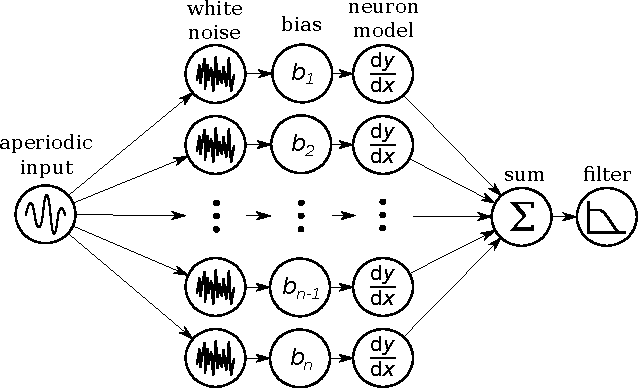
\includegraphics{figure1_experiment.pdf}
  \fi
  \caption{
    \textbf{The experimental setup.} In our experiment, neurons are fed a common aperiodic input. Each neuron also has an independent white noise process and a randomly chosen bias that are added to the input. Varying the amplitude of the noise and the width of the interval from which the biases are randomly drawn allows us to control the amount of noise and heterogeneity in the experiment, respectively. Additionally, some ``off'' neurons invert their input (not shown). The output of each FHN or LIF neuron model is summed and filtered to produce the population output; this is compared with the input signal using mutual information as a metric.
  }
  \label{fig:exp}
\end{figure}

Figure~\ref{fig:infohetero} summarizes the effect of neuronal heterogeneity on the information content of a population of neurons. At low noise levels, we observe a resonance effect in the heterogeneity parameter---there is an optimal level of heterogeneity that maximizes the information content of the population. Furthermore, this optimal level of heterogeneity is around one to two times the root-mean-square amplitude of the input signal. This indicates that optimal heterogeneity corresponds to having neuron firing thresholds that span the full range of input signal values. Too little heterogeneity means that some input signal components cannot be uniquely encoded by the population, since these values will be either well below or well above the firing thresholds of all neurons in the population, and all neurons will fire approximately constantly for these values. Too much heterogeneity results in some neurons that have firing thresholds well below or well above all signal values, causing them to either fire tonically independent of the input signal value, or to fire for no part of the input signal, respectively. This type of resonance in heterogeneity was recently observed by \cite{Mejias2012}, both theoretically and in numerical experiments.

\begin{figure}
  \ifx\hidefigures\undefined
    \centering
    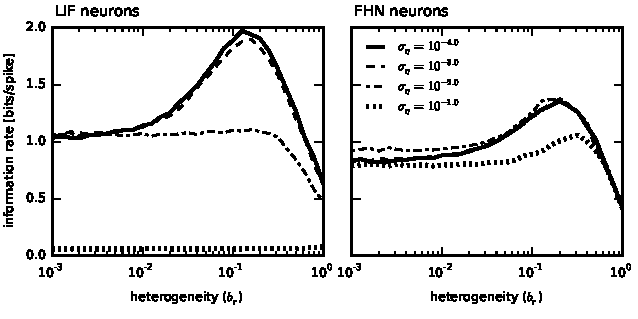
\includegraphics[width=\textwidth]{figure2_infohetero.pdf}
  \fi
  \caption{
    \textbf{Heterogeneity increases information content of a population of neurons, and exhibits a resonance effect.}
    Adding some heterogeneity (x-axis) to a population of LIF or FHN neurons increases their ability to represent an input signal (y-axis), while too much heterogeneity decreases representational ability. This effect is only observed at lower noise levels; at higher levels of noise, the noise alone is able to fully desynchronize neuronal firing and linearize neuron responses, so adding heterogeneity offers no additional benefit.
  }
  \label{fig:infohetero}
\end{figure}

Higher levels of noise reduce or completely eliminate the benefits offered by heterogeneity (Figure~\ref{fig:infohetero}). To examine the interactions between noise and heterogeneity further, we conducted the same experiment across a wide range of noise and heterogeneity values. Figure~\ref{fig:infocontour} illustrates the effects of these interactions on the information content of a population of LIF or FHN neurons. We measured both the absolute information content (in bits) and the information content per spike, or information rate (in bits per spike).

LIF neurons are best able to represent the input signal
with a moderate amount of heterogeneity ($b_r \approx 1.5 \times 10^{-1}$)
and no noise ($\sigma_\eta = 1.0 \times 10^{-4}$).
This was true when measuring both the absolute information content and the information per spike.
FHN neurons, on the other hand, required both heterogeneity and noise
to achieve maximum information content,
because heterogeneity alone is not able to fully desynchronize FHN neurons (see \textsc{\nameref{scn:desync}}).
However, heterogeneity alone was able to maximize the information rate of the system.

We explain this difference between the information content and information rate of FHN neurons
with the fact that noise increases the firing rates of neurons.
While noise offers some benefit to the information content of a population of FHN neurons
(given an optimal level of heterogeneity),
this effect disappears when examining information per spike,
since noise also increases the number of spikes.
In Figure~\ref{fig:infonoise}, we examine more closely the effects of noise on information content and rate in the absence of heterogeneity. Noise shows a clear resonance effect when measuring the absolute information content of the population, but this resonance effect is reduced when measuring the information per spike. We conclude that noise operates partially by increasing the firing rates of neurons, and indeed this effect can be observed when measuring the tuning curves of neurons under noise (see Figure~\ref{fig:tuning}).

The information landscapes of Figure~\ref{fig:infocontour} demonstrate that the effects of noise and heterogeneity are not independent. This is most apparent when examining the absolute information content of LIF populations (top left), and the information rate of FHN populations (bottom right).
For example, LIF neurons show a resonance in heterogeneity in the absence of noise,
but they also show a resonance in noise in the absence of heterogeneity (see also Figure~\ref{fig:infonoise}).
However, if we choose the optimal levels of noise and heterogeneity in the absence of the other factor ($\sigma_\eta \approx 10^{-2}$ and $b_r \approx 2 \times 10^{-1}$), this combined level of noise and heterogeneity does not further increase the information content of the system. This indicates that the effects of noise and heterogeneity are not independent: the optimal level of noise depends on the level of heterogeneity, and vice versa.


\begin{figure}
  \ifx\hidefigures\undefined
    \centering
    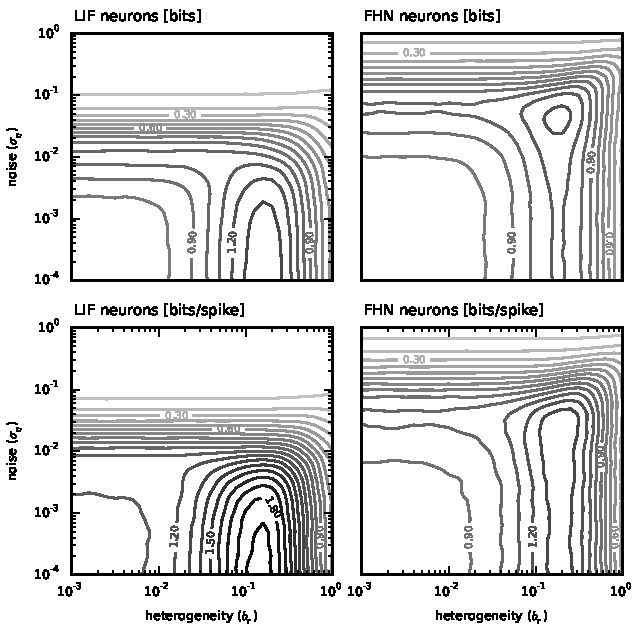
\includegraphics[width=\textwidth]{figure3_infocontour.pdf}
  \fi
  \caption{
    \textbf{The benefits of noise and heterogeneity to information representation are not independent.}
We measured the information content (top, in bits) and information rate (bottom, in bits per spike),
across many levels of noise and heterogeneity.
In LIF neurons, both noise and heterogeneity show independent resonance effects:
given that only one of noise or heterogeneity is present,
there is a non-zero and finite level of noise or heterogeneity that optimizes information content.
Setting both noise and heterogeneity to their (independent) optimal levels
fails to further improve the representational ability of the population,
showing that these effects are not independent.
We propose that both parameters use
the same underlying mechanisms of desynchronization and linearization,
so once the population has been desynchronized and linearized by one parameter,
adding the other cannot further improve information content.
Heterogeneity is unable to fully desynchronize FHN neurons (see \textsc{\nameref{scn:desync}}),
so information content in these neurons is maximized for a specific combination of heterogeneity and noise. However, this effect is not seen when examining the information rate,
indicating that noise benefits neural systems partly through increasing firing rates.
  }
  \label{fig:infocontour}
\end{figure}

\begin{figure}
  \ifx\hidefigures\undefined
    \centering
    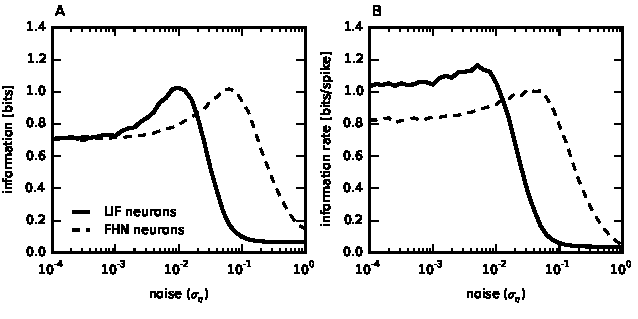
\includegraphics[width=\textwidth]{figure4_infonoise.pdf}
  \fi
  \caption{
    \textbf{Noise increases information content of homogeneous populations of FHN and LIF neurons.} A) In homogeneous populations, noise exhibits a resonance effect on information content. B) The resonance effect of noise is less pronounced when measuring the information rate, indicating that noise operates partially by increasing firing rates.
  }
  \label{fig:infonoise}
\end{figure}

We propose that both noise and heterogeneity improve the information representation ability of a population of neurons by 1) desynchronizing the firing of neurons in the population and 2) linearizing the response of the population to an input signal. These shared mechanisms result in the non-independent interaction between noise and heterogeneity in terms of information content: once either noise or heterogeneity has adequately desynchronized a population, the addition of the other cannot further desynchronize or linearize, and therefore provides no additional increase in information representation. In the following two sections, we present additional experimental results to investigate and quantify the mechanisms of desynchronization and linearization.


\subsection{Desynchronization}
\label{scn:desync}

Consider the following: a group of perfectly homogeneous neurons with no noise, such that their dynamics are completely deterministic. Begun with the same initial conditions, they will follow exactly the same trajectory in phase space because they all receive the same input signal and obey the same set of differential equations. Such a population of simulated neurons will exhibit perfectly synchronized firing events, and therefore the neurons contribute redundant information. Any signal that could be decoded from the firing events of this population of neurons could also be decoded from the spikes of a single neuron. These neurons are perfectly synchronized; at any time, they are all in the same phase of their firing cycle, and in the same position in phase space.

Adding independent noise to each neuron desynchronizes the firing events of the population by causing diffusion of the neuronal phases \citep{Stocks2001a}. A small random perturbation causes a slightly advanced or delayed firing of a neuron, creating a small shift in the phase of that neuron. Specifically, a firing neuron follows a stable limit cycle attractor in phase space; perturbations tangent to the limit cycle result in diffusion along the limit cycle, while perturbations perpendicular to the limit cycle rapidly return the the stable attractor \citep{Tomita1974}. Over time, this diffusion along the limit cycle results in the population of neurons having a wide distribution of phases (Figure~\ref{fig:phase}), and the neurons fire asynchronously (Figure~\ref{fig:syncraster}).

\begin{figure}
  \ifx\hidefigures\undefined
    \centering
    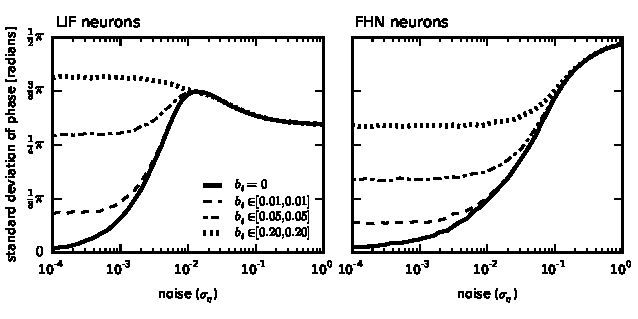
\includegraphics[width=\textwidth]{figure5_phase.pdf}
  \fi
  \caption{
    \textbf{Noise and heterogeneity both desynchronize neurons.} To measure whether noise and heterogeneity have a desynchronizing effect on populations of neurons, we measured the standard deviation of neuron phases across the population (see \textsc{\nameref{scn:methods}}), where a smaller standard deviation indicates increased synchronization. Heterogeneity is seen to significantly desynchronize both FHN and LIF neurons, specifically across low to moderate levels of noise. At high levels of noise, the noise itself is sufficient to desynchronize neurons, and additional heterogeneity has no effect.
  }
  \label{fig:phase}
\end{figure}

\begin{figure}
  \ifx\hidefigures\undefined
    \centering
    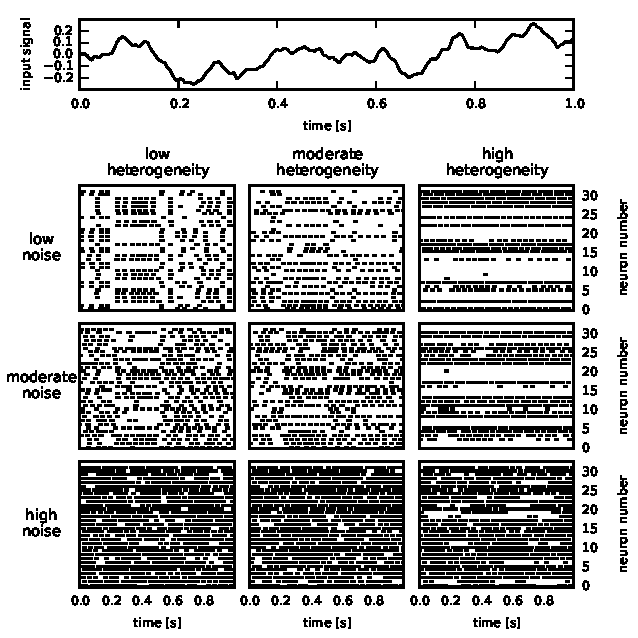
\includegraphics[width=\textwidth]{figure6_syncraster.pdf}
  \fi
  \caption{
    \textbf{The effects of noise and heterogeneity on LIF neuron firing.}
    Spike rasters illustrate the effects of noise and heterogeneity parameters on neuronal firing in a population of 32 LIF neurons. With low noise and heterogeneity, neuronal firing is highly synchronized. Adding a moderate amount of noise or heterogeneity desynchronizes this firing. Adding a moderate level of both parameters cannot provide further desynchronization, since firing is already quite desynchronized. High levels of noise cause rapid firing in almost all neurons, degrading the ability of the population to represent the input signal. High levels of heterogeneity cause the signal to be entirely above or below the firing thresholds of many neurons, again degrading representational ability. Noise: $\sigma_\eta = $$10^{-3}$ (low), $10^{-2}$ (moderate), $10^{-1}$ (high). Heterogeneity: $b_r = $$10^{-2}$ (low), $10^{-1}$ (moderate), $10^{0}$ (high).
  }
  \label{fig:syncraster}
\end{figure}

This previous example is, of course, artificial. It requires that all neurons are \emph{exactly} the same and start with \emph{exactly} the same initial conditions. In a more realistic scenario, one expects that small differences in neuronal parameters or small amounts of noise will cause neurons to desynchronize over a long period of time. This is not the case, because signals below the firing thresholds of a group of neurons have a synchronizing effect on the group. By stopping neuronal firing, these signals push all the neurons in the group towards their stable equilibrium points. When the signal returns to an amplitude above the firing thresholds of neurons in the group, all neurons will begin firing at approximately the same time, and will be once again in phase. Signals with higher frequency components are able to cross larger ranges of firing thresholds in quick succession, and have a stronger synchronizing effect than purely low frequency signals. Thus, more negative (positive) portions of the input signal repeatedly act to synchronize ``on'' (``off'') neurons, and groups of neurons must be able to desynchronize quickly after these synchronization events in order to remain out of phase with one another.

Similar to noise, heterogeneity acts to desynchronize neurons \citep{Burton2012}. Adding heterogeneity to a population increases the range of distribution of neuron phases (Figure~\ref{fig:phase}), thereby desynchronizing populations of both FHN and LIF neurons (Figure~\ref{fig:syncraster}). In a homogeneous population, changes in the input signal cross the common firing threshold of all neurons at the same time, resulting in synchronous firing. Contrast this with a heterogeneous population, where changes in the input signal sequentially cross the thresholds of neurons, causing some to begin firing before others. For example, an increasing input signal will cause neurons with lower thresholds to begin firing before those with higher thresholds, resulting in desynchronized firing within the population of neurons.

High frequency input signals may cross the thresholds of many neurons in a heterogeneous population at the same time, causing a large group of neurons to begin firing simultaneously. LIF neurons are still able to desynchronize quickly after such a stimulus, since the LIF tuning curves used have different firing rates for different sizes of suprathreshold signal (Figure~\ref{fig:tuning}). Specifically, a high-frequency increase in signal amplitude starts neurons firing at approximately the same time, but starts them firing at different rates, allowing them to quickly desynchronize. FHN neurons, however, all have around the same firing rate regardless of the strength of the suprathreshold signal (Figure~\ref{fig:tuning}), and heterogeneity with higher-frequency signals has a reduced effect, since these signals cause many neurons to begin firing at once, unable to desynchronize due to their common firing rate. This discrepancy between LIF and FHN neurons results in heterogeneity having a large effect on phase in LIF neurons (Figure~\ref{fig:phase}A), whereas the desynchronizing effect of heterogeneity in FHN neurons is more modest (Figure~\ref{fig:phase}B).

This difference in the ability of heterogeneity to desynchronize LIF versus FHN neurons
explains why LIF neurons achieve maximum information content with only heterogeneity,
whereas FHN neurons require both heterogeneity and noise (Figure~\ref{fig:infocontour}).
Since heterogeneity does not desynchronize FHN neurons as well as noise does,
adding noise to a heterogeneous population of FHN neurons further desynchronizes them
and increases information content.

\subsection{Linearization}

Intrinsic noise makes neuron tuning curves more linear;
this phenomenon underlies many results in the stochastic resonance literature
\citep{Chialvo1997}.
Noise allows a neuron to respond to input signals below its firing threshold,
by occasionally raising the neuron's membrane voltage high enough
to cross the threshold and trigger an action potential.
This results in a non-zero firing rate for subthreshold signals,
with the firing rate proportional to the strength of the signal.
In type~II neuron models (\emph{e.g.} the FHN model),
noise can also slow firing for signals slightly above the firing threshold,
by momentarily pushing the neuron away from its limit cycle and back to near its unstable equilibrium.
Overall, the addition of noise has the effect
of linearizing the response of the neuron near its firing threshold,
resulting in a smoother transition from the silent to tonic firing regimes (Figure~\ref{fig:tuning}).
This result has been previously observed and extensively studied \citep{Stocks1996,Chialvo1997,Chance2002,Prescott2002,Shu2003}.

\begin{figure}
  \ifx\hidefigures\undefined
    \centering
    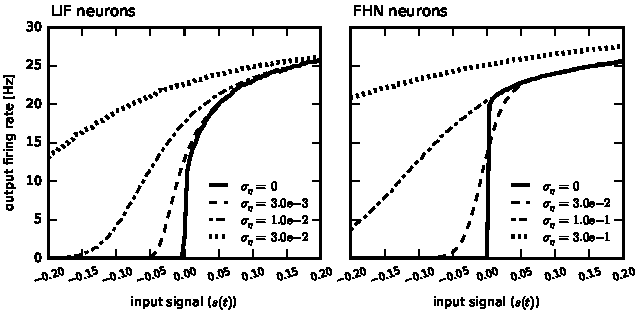
\includegraphics[width=\textwidth]{figure7_tuningnoisy.pdf}
  \fi
  \caption{
    \textbf{Noise linearizes neuron tuning curves.}
    We measured the tuning (stimulus-response) curves of LIF and FHN neurons under various levels of noise.
    We observe that noise linearizes the neuron tuning curves,
    Specifically, noise eliminates the sharp threshold in the tuning curve by
    occasionally pushing the neuron above its firing threshold
    for stimuli that are below the threshold.
    Noise also increases neuron firing rates across some or all stimuli.
  }
  \label{fig:tuning}
\end{figure}

Neuron heterogeneity has a linearizing effect similar to adding noise to a population, but unlike the noisy case, where it made sense to talk about noise linearizing an individual neuron's tuning curve, here we will discuss how heterogeneity linearizes the \emph{population's} tuning curve. The population's tuning curve is the set of points connecting the input signal strength to the decoded output. Since our model uses a simple summing decoder, the population tuning curve is equal to the sum of the individual neuron tuning curves. For a population of neurons with uniformly varied random firing thresholds, the population tuning curve is much more linear than a single neuron's tuning curve, whereas in the homogeneous case the population's tuning curve is the same as the neurons' tuning curve (Figure~\ref{fig:tuninghetero}). The linearizing effect of heterogeneity thereby allows for better representation of an input signal. This result is related to the original idea from \cite{Hubel1962} that variation in neural receptive fields provides a better basis for representing an input signal, and reappears in the recent heterogeneity literature \citep{Angelo2012}.

\begin{figure}
  \ifx\hidefigures\undefined
    \centering
    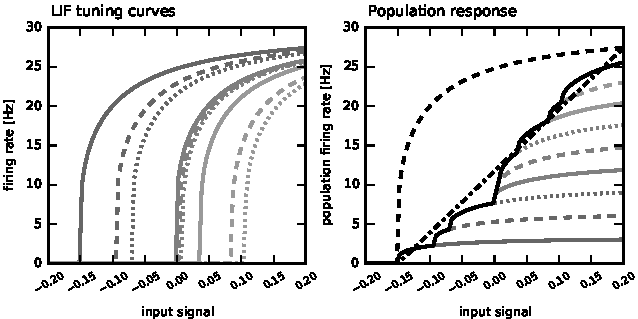
\includegraphics[width=\textwidth]{figure8_tuninghetero.pdf}
  \fi
  \caption{
    \textbf{Heterogeneity linearizes the response of a neuronal population to a stimulus.} A) Tuning curves for a heterogeneous population of $N = 9$ neurons. B) The population response of the heterogeneous population (heavy solid line) is much closer to a linear response (heavy dot-dashed line) than a single LIF tuning curve (heavy dashed line), even though the heterogeneous thresholds are far from evenly spaced.
  }
  \label{fig:tuninghetero}
\end{figure}


%%%%%%%%%%%%%%%%%%%%%%%%%%%%%%%%%%%%%%%%%%%%%%%%%%%%%%%%%%%%%%%%%%%%%%%%%%%%%%%%
\section{Discussion}
\label{scn:discussion}

Our results show that noise and heterogeneity both improve neuronal representation of an input signal, and that these benefits are not independent. Adding noise to a homogeneous neuronal population increases information content, while the same amount of noise degrades information contained by a heterogeneous population (Figures~\ref{fig:infocontour}~and~\ref{fig:infonoise}). This suggests that the benefits of noise and heterogeneity to information content can be explained in terms of shared mechanisms, which we identify as 1) desynchronizing the neurons within a population, and 2) linearizing the response of the population.

The dynamics of a neuron can be viewed as a combination of temporal properties and rate properties. The rate view of neurons treats them as being no more than input-output (or tuning) curves. That is, all temporal dynamics are ignored, and a neuron is reduced to a nonlinear function which turns an input signal into an output signal. The mechanism of linearization affects only the rate properties of neurons, and it is these linearization benefits that are observed in suprathreshold stochastic resonance studies that examine the benefits of noise in populations of binary threshold units \citep{Stocks2000,Stocks2001a,McDonnell2006}. This is because binary threshold units have no temporal properties---they are either on or off depending on the current input signal and noise---and cannot be affected by the temporal benefits of noise. The linearization effects of noise on nonlinear systems have been previously studied (see \cite{Stocks1996} for a review). We have observed that heterogeneity also achieves these linearization effects across a population of neurons, as previously reported by \cite{Eliasmith2003}.

Desynchronization operates by affecting the temporal properties of neuronal firing, and is only observed in spiking neuron models, such as the FHN and LIF models examined in this paper. The output of these models depends not only on the the output firing rate for a given input signal, as determined by the neuron tuning curve, but also by the timing of individual spike events. When nonlinear dynamical models of neurons are examined in a stochastic resonance simulation, as in \cite{Stocks2001}, the results are a combination of the temporally-based desynchronizing and response-time effects of noise, as well as the rate-based linearizing effects of noise.  Desynchronized neurons provide a better temporal basis for representing a signal, since each neuron is able to fire independently and code for a different temporal component of the signal. Even mild correlations between neurons are known to impede a population's representational ability \citep{Zohary1994}.

Our experimental setup was motivated by stochastic resonance experiments such as \cite{Stocks2001}, as well as computational \citep{Brody2003} and experimental \citep{Padmanabhan2010} work looking at heterogeneity. All these experiments present a common input signal to a number of neurons, with added noise or heterogeneity. The common input signal may seem artificial, but it allows us to examine how the properties of individual neurons---including the sign of the input signal (``on'' and ``off'' neurons), the bias current, and the membrane voltage---affect the ability of the neuronal population to encode an input signal. These heterogeneities in the neurons can be viewed as modulating the input signal presented to each neuron, such that each neuron receives a unique input current. In the case of homogeneous populations, all neurons do receive the same input current. This is clearly artificial, and emphasizes why theoreticians should include heterogeneity when modeling neural behaviour.

In our experiments, we saw significantly different results for the LIF neuron model versus the FHN neuron model. Specifically, given an optimal level of heterogeneity, the FHN neurons still benefited from the addition of noise, whereas LIF neurons did not. This raises two questions: why is there a difference between the two models, and does either model better describe the neural systems we wish to study? One way to differentiate between the two models is with bifurcation theory, which classifies the LIF model is a type~I neuron model and the FHN model is a type~II neuron model (though LIF neurons are not prototypical type~I neurons \citep{Mato2008}, they are qualitatively more similar to this category). The difference is that type~I models undergo a saddle-node bifurcation as the input current (the bifurcation parameter) increases, whereas type~II models undergo a subcritical Hopf bifurcation \citep{Mato2008}. Qualitatively, this means that type~I models have continuous tuning curves and can have arbitrarily small firing rates, whereas type~II models have a discontinuity at their firing threshold and when firing cannot fire slower than a given rate. The fact that the LIF model is a type~I neuron model has traditionally made it a better model of cortical neurons \citep{Koch1999}, though studies indicate that some neurons in mammalian (rat) cortex exhibit both type~I and type~II properties \citep{Tateno2004,Tsubo2007}. Previous numerical experiments that have examined stochastic resonance and heterogeneity together have used binary threshold units in their simulations \citep{Stocks2000,McDonnell2006}, which are qualitatively very similar to type~II neurons but without the temporal component. The results of these experiments may have limited applicability to cortical neural systems.

We found that heterogeneity was better able to desynchronize
LIF neurons than FHN neurons (Figure~\ref{fig:phase}),
given that heterogeneity was added only to the firing threshold $b_i$.
We hypothesize that this is due to key differences in the shape of the neuron tuning curves.
The FHN model, being a type~II neuron model,
has a tuning curve that is qualitatively similar to a binary threshold unit,
with a discontinuous increase in firing rate at the firing threshold
and minimal change in firing rate for signals above the threshold (Figure~\ref{fig:tuning}A).
On the other hand, the LIF model, being a type~I neuron model,
has a continuous and monotonically increasing tuning curve,
specifically one that increases smoothly with the strength of a
suprathreshold signal (Figure~\ref{fig:tuning}B).
If a high-frequency signal crosses the firing thresholds of many FHN neurons in quick succession, all the neurons will begin firing both at approximately the same time and with approximately the same rate, taking a long time to desynchronize. With LIF neurons, the high-frequency signal can still cross the firing thresholds of many neurons simultaneously, causing them to begin firing at approximately the same time. However, the signal will result in higher firing rates for neurons with lower firing thresholds than for those with higher firing thresholds, allowing the group of neurons to desynchronize quickly. This key difference between the tuning curves of FHN and LIF neurons results in better desynchronization for LIF neurons.

In our experiments, we added heterogeneity only to the firing threshold $b_i$. While this does capture the variable levels of excitability seen in in vivo neurons \citep{Mejias2012}, due to variations in neuron physiology or differences in the background activity of afferent neurons, there are clearly many other types of heterogeneity in neurons that also deserve attention.
We hypothesize that if heterogeneity were added to other neuron parameters,
the information content of a population of FHN neurons could be optimized without noise, as with LIF neurons.
For example, adding variation to the maximum firing rates of FHN neurons would allow them to desynchronize as quickly as LIF neurons. A system with this level of heterogeneity would require a more complex decoding system than the simple summing neuron model used in this paper, perhaps using the tuning curves to solve for the optimal linear decoders as described by \cite{Salinas1994} or \cite{Eliasmith2003}. Such a decoding scheme could take advantage of a key difference between noise and heterogeneity: The variability produced by heterogeneity is reproducible from trial to trial, whereas the variability due to noise is not. Heterogeneity thereby allows for more complex decoding schemes, such as the combinatorial decoding scheme examined in \cite{Osborne2008}. We leave the extension of heterogeneity to additional neural parameters, and the requisite implementation of more complex decoding schemes, for future work.

Noise and heterogeneity have a fundamental similarity that goes deeper than their mutual ability to increase information transmission in neuronal populations, which is that noise and heterogeneity are both a form of random variation. Specifically, noise corresponds to variation within the phase space (state space) of a system over time, and heterogeneity corresponds to variation within the parameter space of a system across a population. It is important to emphasize that the heterogeneity used in this paper was completely random; the heterogeneous firing thresholds did not have to be specifically chosen or fine-tuned in any way, suggesting that random heterogeneity may be a natural implementation scheme adopted by a biological system like the brain. Finally, in analogy to stochastic resonance with noise, there is a critical level of heterogeneity that optimizes information transmission (Figure~\ref{fig:infohetero}). Noise and heterogeneity should therefore be thought of as analogous mechanisms, but in different parts of the neuronal model (the state space versus the parameter space, respectively).

Despite the similarities between noise and heterogeneity, there are also considerable differences.
Perhaps the most important is that the response of a heterogeneous population is reproducible from trial to trial, whereas the response of a noisy population is only reproducible on average.
Though we do not examine this effect here, due to our simplistic decoding method,
many authors have commented the prevalence of reproducibility in neural systems \citep[e.g.,][]{Mainen1995}.
Another significant difference between noise and heterogeneity is that noise increases the firing rate of neurons, whereas heterogeneity does not (on average). This results in noise being beneficial to the absolute information content of a population, but having a reduced effect on the information per spike (Figure~\ref{fig:infonoise}).
A third difference is that under some conditions (LIF neurons) heterogeneity alone is able to optimize information content, whereas under others (FHN neurons) both heterogeneity and noise are required.

Both our results here and the results of numerous other researchers suggest that noise and heterogeneity may be important vehicles used by neural systems to optimize information flow.
Yet the extent to which actual biological neural systems exploit either heterogeneity or stochastic resonance for improved information encoding and transmission remains unclear.
A number of recent studies show that heterogeneity can be very important in encoding sensory information, such as for certain electric fishes \citep{Marsat2010} or in the rodent olfactory system \citep{Padmanabhan2010,Burton2012}. Another recent study shows stochastic resonance effects in human auditory cortex, specifically that noise can increase correlation both within and between some cortical regions \citep{Ward2010}. More studies of this nature are required to determine both what neural systems show evidence of heterogeneity or stochastic resonance, and more importantly, whether these systems actually take advantage of them for improved population coding.
The differences between noise and heterogeneity suggest that the extent to which they are exploited may vary significantly from one neural system to another, depending on the physiology of the neurons involved and whether factors like firing rate are a significant constraint.
The work presented here demonstrates the complex interaction between noise and heterogeneity due to the shared underlying mechanisms of desynchronization and linearization, and explains how these mechanisms lead to improved information processing characteristics.


%%%%%%%%%%%%%%%%%%%%%%%%%%%%%%%%%%%%%%%%%%%%%%%%%%%%%%%%%%%%%%%%%%%%%%%%%%%%%%%%
\section{Models and Methods}
\label{scn:methods}

Our model consists of an input signal $s(t)$ encoded by a population of neurons, specifically having the same signal injected into the soma of all cells in the population (see Equations~\ref{eqn:fhn}~and~\ref{eqn:lif}). We ran simulations using both the FitzHugh-Nagumo (FHN) neuron model and the leaky integrate-and-fire (LIF) neuron model. Signal decoding is modeled by summing the spikes of each neuron in the population and low-pass filtering the result to obtain the output signal $r(t)$. This is analogous to determining the somatic current of a single receiving neuron, where the filtering is performed by synapses. The input and output signals are then compared using mutual information, to measure how well the output signal encodes the input signal. Independent and identically distributed (i.i.d.) additive Gaussian noise processes are added to each neuron, with standard deviation $\sigma_\eta$ used to modulate the noise level in each experiment. Heterogeneity is also added by choosing neuron biases $b_i$ from a random uniform distribution, where the width of the distribution controls the degree of heterogeneity.

\textbf{FitzHugh-Nagumo (FHN) model.} The FHN model is a simplification of the Hodgkin-Huxley model \citep{FitzHugh1961}. We chose to use the standard formulation presented by \cite{Izhikevich2006}, given for the $i$-th neuron by two coupled ordinary differential equations:
\begin{equation}
  \begin{array}{rl}
    \dot{v_i} & = v_i - \frac{1}{3}v_i^3 - w_i + \beta_i + e_i s(t) + \eta_i(t) \vspace{1em}\\
    \dot{w_i} & = 0.08(v_i - 0.8w_i + 0.7),
  \end{array}
  \label{eqn:fhn}
\end{equation}
where $v_i(t)$ is a fast (voltage) variable, $w_i(t)$ is a slow (recovery) variable, $\beta_i$ is a constant bias voltage, $e_i$ is a simple encoder equal to 1 for ``on'' neurons and $-1$ for ``off'' neurons, $s(t)$ is an input signal common to all neurons, and $\eta_i(t)$ is a Gaussian white noise process with autocorrelation $\left<\eta_i(t)\eta_j(t + \tau)\right> = \sigma^2 \delta_{ij}\delta(\tau)$. We chose $\beta_i = 0.3216 - b_i$, with the offset 0.3216 chosen such that the bias $b_i$ corresponds to the threshold at which the neuron begins firing.

Originally, we took the FHN neuron output to be equal to the positive part of the membrane voltage.
This resulted in spikes that were not discrete, stereotyped events,
but rather extended events that could transmit information in their amplitude.
Although some researchers have argued that in vivo neurons do transmit information in spike amplitude,
we found that this approach did not provide sensible results when the FHN model
was pushed to the limits of its operating range,
specifically for high levels of noise and wide ranges of heterogeneity.

We therefore developed a basic method to determine when the FHN model was spiking,
and transmitting an instantaneous stereotyped spike when this occurred.
The FHN neuron model was considered to spike
when the voltage was above the threshold $V_{th} = 0$ for a time of 1 ms,
and was not allowed to spike again until the voltage was below the threshold for 1 ms.
This 1 ms buffer time was necessary so that brief membrane voltage threshold crossings
due to noise were not counted as spikes.

\textbf{Leaky integrate-and-fire (LIF) model.} The LIF model describes a neuron as a membrane with resistance $R$ and capacitance $C$, which fires spikes when the membrane voltage $v(t)$ crosses the threshold $V_{th}$. It is governed by the differential equation
\begin{equation}
  \tau_{RC} \dot{v_i} = -v_i + \beta_i + \alpha \left( e_i s(t) + \eta_i(t) \right),
  \label{eqn:lif}
\end{equation}
where $v_i(t)$ is the membrane voltage, $\tau_{RC} = RC$ is the membrane time constant, $\alpha$ is the input signal gain, $\beta_i$ is a constant bias voltage, $\eta_i(t)$ is a delta-correlated Gaussian white noise process (as with the FHN neuron model), and $s(t)$ is an input signal common to all neurons. When a neuron voltage reaches the threshold voltage $V_{th} = 1$, the neuron fires a spike and begins a refractory period. The length of the refractory period is given by the refractory time constant $\tau_{ref}$, and during this time the neuron voltage is held at zero. Once the refractory period is finished, the neuron obeys Equation~\ref{eqn:lif} until another spike occurs.

We chose $\tau_{RC}$ to be 20 ms, which is typical for cortical neurons \citep{McCormick1985}. We then chose $\tau_{ref}$ to be 33 ms, thus giving a maximum firing rate (30 Hz) approximately the same as the FHN model. We chose $\alpha$ to be 15, to achieve a similar maximum firing rate to the FHN model over the range of inputs used. We chose $\beta_i = V_{th} - \alpha b_i$, such that $b_i$ is a bias that corresponds to the threshold at which the neuron begins firing.


\textbf{Input signal generation.} The input signal consisted of Gaussian white noise filtered with an $\alpha$ function, $\alpha(t) = (t / \tau_c) e^{-t / \tau_c}$, which models synaptic firing \citep{Galan2008}. The signal was normalized to have zero-mean and a standard deviation of $\sigma_s = 0.1$. The correlation time was chosen to be $\tau_c = 20$ ms, which is on the upper end of the times used by \cite{Mainen1995}. This correlation time results in a cutoff frequency of $f_c = 7.96$ Hz, which is considerably lower than the maximum firing rate of the neurons ($\sim 25$ Hz).


\textbf{Output signal decoding.} To determine the output signal $r(t)$, we used the basic model of a summing neuron similar to the one proposed by \cite{Stocks2001}. Specifically, the output signal $r$ is given by
\begin{equation}
  \tau \dot{r} = -r + \sum\limits_{i=1}^N s_i(t)
\end{equation}
where $N$ is the number of neurons in the encoding population, and $s_i(t_j)$ is 1 if neuron $i$ is spiking at time $t_j$ and 0 otherwise. This model simulates a summing neuron which only receives discrete, stereotyped spikes from input neurons, and then low-pass filters and sums these spikes.
We chose a time constant $\tau = 20$ ms for the filter. This value was chosen to optimize the information throughput of the system; it does so likely because it is the same as the correlation time of the input signal. Other choices of the filter time constant produce the same qualitative results, but with lower levels of information content.


\textbf{Mutual information.} We use Shannon mutual-information as the measure of similarity between the input and output signal \citep{Heneghan1996,Stocks2001}, where the mutual information $I$ (in bits) between the output signal $r$ and input signal $s$ is given by
\begin{equation}
  I(s,r) = \sum\limits_{s \in S} \sum\limits_{r \in R} p(s,r) \log_2\left(\frac{p(s,r)}{p(s)p(r)}\right),
\end{equation}
where $S$ is the domain of the input signal $s(t)$ and $R$ is the domain of the output signal $r(t)$. To compute the joint probability distribution $p(s,r)$ for discrete signals $s(t)$ and $r(t)$, the domains $S$ and $R$ are each divided into equal bins, and a joint histogram of the points $[s(t_i),r(t_i)]$ is formed. This histogram is used to approximate the joint probability function $p(s,r)$ by scaling it so the sum across all $s$ and $r$ is unity (\emph{i.e.,} dividing the histogram by the total number of points $N$). For all simulations, we divided the domains $S$ and $R$ into 19 bins each.

One shortfall of this comparison method is that it does not account for the delay between the input and output signals, due to the non-zero reaction time of the neurons. In neural systems, some delay is to be expected, and we should not penalize our simulated networks for not being able to encode and decode an input signal instantaneously. The difficulty in comparing a delayed version of the input signal with the output signal is that it raises the question of what length of delay should be used. Each pair of noise and heterogeneity levels may conceivably have a unique optimal delay, and in order to not favor either noise or heterogeneity, the optimal delay (\emph{i.e.,} the delay that produces the highest mutual information) should be calculated and used at each pair of noise and heterogeneity levels. In the interest of simplicity, we decided to instead compare the input and output signals with no delay, as is consistent with previous experiments \citep{Stocks2001}.

We obtain the information per spike by multiplying the mutual information by the Nyquist rate of the signal (2 times the signal bandwidth of $f_c = 7.96$ Hz). This results in an information rate (in bits per second), which we then divide by the average number of spikes per second of a neuron in the population, to obtain the information per spike.

\textbf{Heterogeneity.} To introduce heterogeneity into the population, we varied the bias voltages of the neurons. In homogeneous populations, all neurons had bias voltages equal to zero, the mean of the input signal. Heterogeneous populations had neurons with uniformly randomly distributed biases chosen from a range centered around the mean. In particular, three ranges were used: $[-0.01,0.01]$, $[-0.05,0.05]$, and $[-0.2,0.2]$, corresponding to small, medium and large levels of heterogeneity. The ranges were chosen to be roughly logarithmically distributed, with the largest range corresponding to biases that covered two standard deviations of the input signal.

\textbf{``On'' and ``off'' neurons.} To help minimize subthreshold stochastic resonance effects from significantly contributing to our results, we used populations that contained an equal number of ``on'' and ``off'' neurons, \emph{i.e.,} neurons that both increase firing rates as the input signal increases, and increase firing rates as the signal decreases. In terms of our model, this means that half the neurons of each population had $e_i = 1$, and the other half had $e_i = -1$. This means that half the population represents the positive and negative parts of the signal, respectively, and only a small amount of information is gained by the subthreshold SR effect, which allows each half of the population to represent both positive and negative signal components.

\textbf{Population phase.} To determine how synchronous a population of neurons was, we measured the standard deviation of the neuron phases around the mean population phase. FHN neuron phases were determined by measuring the angle of the $(V(t),W(t))$ point in phase space around a central point, chosen to be $(-0.22,0.60)$ since this lies roughly in the center of the FHN limit cycle. For LIF neurons, the refractory period was scaled to correspond to the first $180^\circ$ of phase, and if the neuron was out of the refractory period, the phase was computed as $180^\circ ( 1 + \max(0,\min(1,V(t))) )$. The mean phase $\bar\theta$ was computed as
\begin{equation}
  \bar\theta(t) = \tan^{-1} \left( \frac{1}{N}\sum\limits_{i=1}^N \cos\theta_i(t),
                                  \frac{1}{N}\sum\limits_{i=1}^N \sin\theta_i(t) \right),
\end{equation}
where $\theta_i(t)$ is the phase of neuron $i$ at time $t$, $N$ is the number of neurons in the population, and $\alpha = \tan^{-1}(x,y)$ is the two-argument arctangent function such that $\tan\alpha = y/x$. The standard deviation $\theta_\sigma(t)$ of the population phase is then given by
\begin{equation}
  \theta_\sigma(t) = \sqrt{ \frac{1}{N} \sum\limits_{i=1}^N (\mathrm{wrap}(\theta_i - \bar\theta))^2 },
\end{equation}
where the function $\mathrm{wrap}(\alpha) = (\alpha + \pi \mod 2\pi) - \pi$ converts the angle $\alpha$ to its equivalent angle in the range $[-\pi,\pi)$. Figure~\ref{fig:phase} presents the mean over all simulation time of the standard deviation of the phase.

\textbf{Simulation details.} The information transmission plots with a noise axis (Figures~\ref{fig:infocontour}~and~\ref{fig:infonoise}) were computed using noise levels in the range $\sigma_\eta \in [10^{-4},1]$, with the levels logarithmically spaced in steps of $10^{0.1}$. We chose the low end of these ranges to be an insignificant level of noise---where information content qualitatively the same as the noise-free case---and increasing until the noise completely overpowered the signal such that only a negligible amount of signal information could be recovered. For information plots with a heterogeneity axis (Figures~\ref{fig:infohetero}~and~\ref{fig:infocontour}), we chose $b_r \in [10^{-3}, 1]$, with points logarithmically spaced in steps of $10^{0.1}$. Again, the low end of this range corresponds to an insignificant level of heterogeneity (qualitatively the same as the homogeneous case), and the high end corresponds to the case where either information content reduced to insignificant levels (LIF neurons), or firing thresholds were so extreme that increasing them further would push the neuron model outside its valid range of operation (FHN neurons).

At each combination of noise and heterogeneity levels, 100 simulations were performed, each having a simulation time of 4.5 seconds, with the first 0.5 seconds of each simulation being discarded to allow any transients created by the initial conditions to settle. A time step of $\Delta t = 10^{-4}$ was used. For each simulation, new sets of both random biases $b_i$ and noise $\eta_i(t)$ were generated for each neuron. The final traces in the figures show the mean over all simulations. The standard error of the mean at each point was not plotted because it was small in all cases, with statistically significant differences between the traces.

The tuning curve plots (Figure~\ref{fig:tuning}) were all calculated empirically by measuring the firing rate of simulated neurons. The range of inputs measured was $[-0.2, 0.2]$, divided into 51 equally spaced points (intervals of $0.008$). At each point, a constant signal at that input value was presented to $N = 30$ identical neurons, with a duration of 5.5 seconds. The first 0.5 seconds of neuron output was discarded, to reduce the effects of initial condition transients, and the average spike rate for each neuron over the remaining time period was calculated.
The tuning curves presented in the plots show the average firing rate of all $N = 30$ neurons for each input value.

\subsection*{Acknowledgments}

We thank the anonymous reviewers for their detailed and thoughtful comments, which greatly improved the quality of the manuscript.
We also thank Jeff Orchard and Matthew S. Wilson for feedback on earlier drafts of the manuscript.


\begin{thebibliography}{}

\bibitem[Angelo et~al., 2012]{Angelo2012}
Angelo, K., Rancz, E.~a., Pimentel, D., Hundahl, C., Hannibal, J., Fleischmann,
  A., Pichler, B., and Margrie, T.~W. (2012).
\newblock {A biophysical signature of network affiliation and sensory
  processing in mitral cells}.
\newblock {\em Nature}, 488(7411):375--8.

\bibitem[Brody and Hopfield, 2003]{Brody2003}
Brody, C.~D. and Hopfield, J.~J. (2003).
\newblock {Simple networks for spike-timing-based computation, with application
  to olfactory processing.}
\newblock {\em Neuron}, 37(5):843--52.

\bibitem[Burton et~al., 2012]{Burton2012}
Burton, S.~D., Ermentrout, G.~B., and Urban, N.~N. (2012).
\newblock {Intrinsic heterogeneity in oscillatory dynamics limits
  correlation-induced neural synchronization.}
\newblock {\em Journal of neurophysiology}, 108(8):2115--33.

\bibitem[Chance et~al., 2002]{Chance2002}
Chance, F.~S., Abbott, L.~F., and Reyes, A.~D. (2002).
\newblock {Gain modulation from background synaptic input.}
\newblock {\em Neuron}, 35(4):773--82.

\bibitem[Chelaru and Dragoi, 2008]{Chelaru2008}
Chelaru, M.~I. and Dragoi, V. (2008).
\newblock {Efficient coding in heterogeneous neuronal populations.}
\newblock {\em Proceedings of the National Academy of Sciences},
  105(42):16344--9.

\bibitem[Chialvo et~al., 1997]{Chialvo1997}
Chialvo, D., Longtin, A., and M\"{u}ller-Gerking, J. (1997).
\newblock {Stochastic resonance in models of neuronal ensembles}.
\newblock {\em Physical Review E}, 55(2):1798--1808.

\bibitem[Collins et~al., 1995]{Collins1995}
Collins, J.~J., Chow, C.~C., and Imhoff, T.~T. (1995).
\newblock {Stochastic resonance without tuning}.
\newblock {\em Nature}, 376:236--238.

\bibitem[Ecker et~al., 2011]{Ecker2011}
Ecker, A.~S., Berens, P., Tolias, A.~S., and Bethge, M. (2011).
\newblock {The effect of noise correlations in populations of diversely tuned
  neurons.}
\newblock {\em The Journal of Neuroscience}, 31(40):14272--83.

\bibitem[Eliasmith and Anderson, 2003]{Eliasmith2003}
Eliasmith, C. and Anderson, C.~H. (2003).
\newblock {\em {Neural Engineering: Computation, Representation, and Dynamics
  in Neurobiological Systems}}.
\newblock MIT Press, Cambridge, MA.

\bibitem[Fitzhugh, 1961]{FitzHugh1961}
Fitzhugh, R. (1961).
\newblock {Impulses and physiological states in theoretical models of nerve
  membrane}.
\newblock {\em Biophysical journal}, 1(1948):445--466.

\bibitem[Gal\'{a}n et~al., 2008]{Galan2008}
Gal\'{a}n, R.~F., Ermentrout, G.~B., and Urban, N.~N. (2008).
\newblock {Optimal time scale for spike-time reliability: theory, simulations,
  and experiments.}
\newblock {\em Journal of neurophysiology}, 99(1):277--83.

\bibitem[Gammaitoni et~al., 1998]{Gammaitoni1998}
Gammaitoni, L., H\"{a}nggi, P., Jung, P., and Marchesoni, F. (1998).
\newblock {Stochastic resonance}.
\newblock {\em Reviews of Modern Physics}, 70(1):223--287.

\bibitem[Heneghan et~al., 1996]{Heneghan1996}
Heneghan, C., Chow, C., Collins, J.~J., Imhoff, T.~T., Lowen, S.~B., and Teich,
  M.~C. (1996).
\newblock {Information measures quantifying aperiodic stochastic resonance.}
\newblock {\em Physical Review E}, 54(3):R2228--R2231.

\bibitem[Hubel and Wiesel, 1962]{Hubel1962}
Hubel, D. and Wiesel, T. (1962).
\newblock {Receptive fields, binocular interaction and functional architecture
  in the cat's visual cortex}.
\newblock {\em The Journal of physiology}, 160:106--154.

\bibitem[Izhikevich and FitzHugh, 2006]{Izhikevich2006}
Izhikevich, E.~M. and FitzHugh, R. (2006).
\newblock {FitzHugh-Nagumo model}.
\newblock {\em Scholarpedia}, 1(9):1349.

\bibitem[Koch, 1999]{Koch1999}
Koch, C. (1999).
\newblock {\em {Biophysics of computation: Information processing in single
  neurons}}.
\newblock Oxford University Press, New York, NY.

\bibitem[Longtin and Chialvo, 1998]{Longtin1998}
Longtin, A. and Chialvo, D.~R. (1998).
\newblock {Stochastic and Deterministic Resonances for Excitable Systems}.
\newblock {\em Physical Review Letters}, 81(18):4012--4015.

\bibitem[Mainen and Sejnowski, 1995]{Mainen1995}
Mainen, Z.~F. and Sejnowski, T.~J. (1995).
\newblock {Reliability of spike timing in neocortical neurons.}
\newblock {\em Science (New York, N.Y.)}, 268(5216):1503--6.

\bibitem[Marsat and Maler, 2010]{Marsat2010}
Marsat, G. and Maler, L. (2010).
\newblock {Neural heterogeneity and efficient population codes for
  communication signals.}
\newblock {\em Journal of neurophysiology}, 104(5):2543--55.

\bibitem[Mato and Samengo, 2008]{Mato2008}
Mato, G. and Samengo, I. (2008).
\newblock {Type I and type II neuron models are selectively driven by
  differential stimulus features}.
\newblock {\em Neural Computation}, 2440:2418--2440.

\bibitem[McCormick et~al., 1985]{McCormick1985}
McCormick, D.~A., Connors, B.~W., Lighthall, J.~W., and Prince, D.~A. (1985).
\newblock {Comparative electrophysiology of pyramidal and sparsely spiny
  stellate neurons of the neocortex}.
\newblock {\em Journal of Neurophysiology}, 54:782--806.

\bibitem[McDonnell and Abbott, 2009]{McDonnell2009}
McDonnell, M.~D. and Abbott, D. (2009).
\newblock {What is stochastic resonance? Definitions, misconceptions, debates,
  and its relevance to biology.}
\newblock {\em PLoS Computational Biology}, 5(5):e1000348.

\bibitem[McDonnell et~al., 2006]{McDonnell2006}
McDonnell, M.~D., Stocks, N.~G., Pearce, C.~E., and Abbott, D. (2006).
\newblock {Optimal information transmission in nonlinear arrays through
  suprathreshold stochastic resonance}.
\newblock {\em Physics Letters A}, 352(3):183--189.

\bibitem[McDonnell and Ward, 2011]{McDonnell2011}
McDonnell, M.~D. and Ward, L.~M. (2011).
\newblock {The benefits of noise in neural systems: bridging theory and
  experiment}.
\newblock {\em Nature Reviews Neuroscience}, 12(7):415--426.

\bibitem[Mejias and Longtin, 2012]{Mejias2012}
Mejias, J. and Longtin, A. (2012).
\newblock {Optimal Heterogeneity for Coding in Spiking Neural Networks}.
\newblock {\em Physical Review Letters}, 108(22):228102.

\bibitem[Osborne et~al., 2008]{Osborne2008}
Osborne, L.~C., Palmer, S.~E., Lisberger, S.~G., and Bialek, W. (2008).
\newblock {The neural basis for combinatorial coding in a cortical population
  response.}
\newblock {\em The Journal of Neuroscience}, 28(50):13522--31.

\bibitem[Padmanabhan and Urban, 2010]{Padmanabhan2010}
Padmanabhan, K. and Urban, N.~N. (2010).
\newblock {Intrinsic biophysical diversity decorrelates neuronal firing while
  increasing information content.}
\newblock {\em Nature Neuroscience}, 13(10):1276--82.

\bibitem[Prescott and {De Koninck}, 2002]{Prescott2002}
Prescott, S.~a. and {De Koninck}, Y. (2002).
\newblock {Gain control of firing rate by shunting inhibition: roles of
  synaptic noise and dendritic saturation.}
\newblock {\em Proceedings of the National Academy of Sciences},
  100(4):2076--81.

\bibitem[Salinas and Abbott, 1994]{Salinas1994}
Salinas, E. and Abbott, L. (1994).
\newblock {Vector reconstruction from firing rates}.
\newblock {\em Journal of computational neuroscience}, 1(1):89--107.

\bibitem[Shamir and Sompolinsky, 2006]{Shamir2006}
Shamir, M. and Sompolinsky, H. (2006).
\newblock {Implications of neuronal diversity on population coding.}
\newblock {\em Neural Computation}, 18(8):1951--86.

\bibitem[Shu et~al., 2003]{Shu2003}
Shu, Y., Hasenstaub, A., Badoual, M., Bal, T., and McCormick, D.~a. (2003).
\newblock {Barrages of synaptic activity control the gain and sensitivity of
  cortical neurons.}
\newblock {\em The Journal of Neuroscience}, 23(32):10388--401.

\bibitem[Stocks, 2000]{Stocks2000}
Stocks, N.~G. (2000).
\newblock {Suprathreshold stochastic resonance in multilevel threshold
  systems}.
\newblock {\em Physical review letters}, 84(11):2310--3.

\bibitem[Stocks, 2001]{Stocks2001a}
Stocks, N.~G. (2001).
\newblock {Information transmission in parallel threshold arrays:
  Suprathreshold stochastic resonance}.
\newblock {\em Physical Review E}, 63(4):1--9.

\bibitem[Stocks and Mannella, 2001]{Stocks2001}
Stocks, N.~G. and Mannella, R. (2001).
\newblock {Generic noise-enhanced coding in neuronal arrays}.
\newblock {\em Physical Review E}, 64:030902.

\bibitem[Stocks et~al., 1996]{Stocks1996}
Stocks, N.~G., Stein, N., Short, H., Mannella, R., Luchinsky, D., McClintock,
  P., and Dykman, M. (1996).
\newblock {Noise-induced linearization and delinearization}.
\newblock In {\em Fluctuations and Order}, pages 53--67.

\bibitem[Tateno et~al., 2004]{Tateno2004}
Tateno, T., Harsch, a., and Robinson, H. P.~C. (2004).
\newblock {Threshold firing frequency-current relationships of neurons in rat
  somatosensory cortex: type 1 and type 2 dynamics.}
\newblock {\em Journal of neurophysiology}, 92(4):2283--94.

\bibitem[Tomita et~al., 1974]{Tomita1974}
Tomita, K., Ohta, T., and Tomita, H. (1974).
\newblock {Irreversible circulation and orbital revolution}.
\newblock {\em Prog. Theor. Phys}, 52(6):1744--1765.

\bibitem[Tsubo et~al., 2007]{Tsubo2007}
Tsubo, Y., Takada, M., Reyes, A.~D., and Fukai, T. (2007).
\newblock {Layer and frequency dependencies of phase response properties of
  pyramidal neurons in rat motor cortex.}
\newblock {\em The European journal of neuroscience}, 25(11):3429--41.

\bibitem[Ward et~al., 2010]{Ward2010}
Ward, L.~M., MacLean, S.~E., and Kirschner, A. (2010).
\newblock {Stochastic Resonance Modulates Neural Synchronization within and
  between Cortical Sources}.
\newblock {\em PLoS ONE}, 5(12):e14371.

\bibitem[Wiesenfeld et~al., 1994]{Wiesenfeld1994}
Wiesenfeld, K., Pierson, D., and Pantazelou, E. (1994).
\newblock {Stochastic resonance on a circle}.
\newblock {\em Physical Review Letters}, 72(14):2125--2129.

\bibitem[Zohary et~al., 1994]{Zohary1994}
Zohary, E., Shadlen, M., and Newsome, W. (1994).
\newblock {Correlated neuronal discharge rate and its implications for
  psychophysical performance}.
\newblock {\em Nature}, 370:140--143.

\end{thebibliography}

\end{document}
